% !TEX program = pdflatex
% Artículo: Más brecha que efecto (PISA 2025, Argentina)
% Compilación: latexmk -pdf main.tex   (ver paper/README.md)
\documentclass[11pt,a4paper]{article}

% ---------- Codificación, idioma y tipografía ----------
\usepackage[T1]{fontenc}
\usepackage[utf8]{inputenc}
\usepackage[spanish,es-tabla,es-nodecimaldot,es-noshorthands]{babel}
\usepackage[sc]{mathpazo}
\linespread{1.06}
\usepackage[final]{microtype}
\usepackage{csquotes}
\usepackage[htt]{hyphenat}
\emergencystretch=2.5em

% ---------- Página ----------
\usepackage[a4paper,top=2.6cm,bottom=2.7cm,left=2.6cm,right=2.6cm,headheight=14pt]{geometry}
\usepackage{fancyhdr}
\pagestyle{fancy}
\fancyhf{}
\fancyhead[L]{\small\textsc{N. Urday Quiroga}}
\fancyhead[R]{\small\textit{Más brecha que efecto: IA y desigualdad en PISA 2025}}
\fancyfoot[C]{\small\thepage}
\renewcommand{\headrulewidth}{0.3pt}

% ---------- Matemática, tablas, figuras ----------
\usepackage{amsmath,amssymb,bm}
\usepackage{booktabs,tabularx,array,threeparttable}
\usepackage{graphicx}
\usepackage[dvipsnames]{xcolor}
\usepackage{tikz}
\usetikzlibrary{positioning,arrows.meta,calc}
\usepackage{enumitem}
\setlist{itemsep=2pt,topsep=4pt}
\setlength{\tabcolsep}{4.5pt}
\usepackage[font=small,labelfont=bf,labelsep=period,justification=justified,singlelinecheck=false]{caption}
\usepackage{titlesec}
\definecolor{azul}{HTML}{1F5FA8}
\definecolor{gristexto}{HTML}{555555}
\titleformat{\section}{\large\bfseries\color{azul}}{\thesection.}{0.6em}{}
\titleformat{\subsection}{\normalsize\bfseries}{\thesubsection.}{0.5em}{}
\titleformat{\subsubsection}[runin]{\normalsize\itshape}{}{0em}{}[.]
\titlespacing*{\section}{0pt}{1.6\baselineskip}{0.6\baselineskip}
\titlespacing*{\subsection}{0pt}{1.1\baselineskip}{0.4\baselineskip}

% ---------- Bibliografía ----------
\usepackage[backend=bibtex,style=authoryear,maxcitenames=2,maxbibnames=8,giveninits=true,
            uniquename=init,doi=true,url=true,isbn=false,natbib=true]{biblatex}
\addbibresource{referencias.bib}
\renewcommand*{\bibfont}{\small}

\usepackage[colorlinks=true,linkcolor=azul,citecolor=azul,urlcolor=azul,
            pdftitle={Más brecha que efecto: nivel socioeconómico, uso de chatbots de inteligencia artificial y rendimiento escolar en Argentina (PISA 2025)},
            pdfauthor={Nazareno Urday Quiroga}]{hyperref}

% ---------- Macros ----------
\newcommand{\pendiente}[1]{\textcolor{BrickRed}{\textbf{[Pendiente del autor: #1]}}}
\newcommand{\var}[1]{\texttt{#1}}
\newcommand{\nb}[1]{\texttt{\small notebooks/#1}}
\newcommand{\arch}[1]{\texttt{\small #1}}
\newcommand{\E}{\operatorname{E}}
\newcommand{\V}{\widehat{V}}
\newcommand{\ee}{\operatorname{ee}}
\newcommand{\pp}{\,p.p.}
\newcommand{\ic}[2]{IC\,95\,\%: #1 a #2}
\DeclareMathOperator*{\argmin}{arg\,min}
\makeatletter\newcommand{\filas}[1]{\@@input tablas/#1.tex }\makeatother % \input expandible, compatible con booktabs

\begin{document}

% =====================================================================
\thispagestyle{plain}
\vspace*{-0.6cm}
\noindent{\color{azul}\rule{\textwidth}{1.2pt}}\par\vspace{0.6cm}
\noindent{\LARGE\bfseries Más brecha que efecto\par}
\vspace{0.35cm}
\noindent{\Large Nivel socioeconómico, uso de chatbots de inteligencia artificial y rendimiento escolar en Argentina: evidencia asociativa con diseño muestral complejo a partir de PISA~2025\par}
\vspace{0.6cm}
\noindent{\color{azul}\rule{\textwidth}{0.4pt}}\par\vspace{0.7cm}
\noindent{\large Nazareno Urday Quiroga}\par
\vspace{0.15cm}
\noindent{\small\color{gristexto} Versión de trabajo para revisión del autor, 16 de noviembre de 2026}\par
\vspace{0.9cm}

\noindent\textbf{Resumen}\par\smallskip
\noindent\small
\textbf{Objetivo.} Estimar cómo se asocian el nivel socioeconómico y la frecuencia de uso de chatbots de inteligencia artificial (IA) con el rendimiento de los estudiantes de 15 años de Argentina, y delimitar qué permiten afirmar los datos.
\textbf{Método.} Análisis secundario, transversal, del archivo de estudiantes de PISA~2025 (11.092 estudiantes, 412 escuelas). Todas las estimaciones usan el peso final, los 80 pesos replicados (replicación repetida balanceada con factor de Fay 0,5, supuesto heredado de ciclos anteriores) y los 10 valores plausibles combinados con las reglas de Rubin. Cinco hipótesis se fijaron antes del análisis (H1--H5) y cuatro se declaran exploratorias (HC1--HC4).
\textbf{Resultados.} Cada unidad del índice ESCS se asocia con 30,6 puntos más en ciencias (\ic{26,3}{34,8}); el cuartil superior supera al inferior en 82,4 puntos. Entre quienes respondieron, el cuartil superior de ESCS usa IA semanal o diariamente entre 13,3 y 16,9 puntos porcentuales más, según la actividad. Sin ajustar, el uso frecuente frente a ninguno se asocia con $+$28,4 puntos al investigar un tema, $+$26,6 al ayudar a aprender y $+$18,8 al resumir, y con una diferencia no concluyente al redactar borradores ($+$7,1; \ic{$-$3,0}{17,2}). Al ajustar por ESCS, sexo y grado, el coeficiente de la frecuencia media cae de 9,5 a 4,0 puntos por punto de escala (\ic{1,1}{6,9}). El 29\,\% de los estudiantes que recibieron las preguntas de IA no las respondió, y rinde 66,0 puntos menos (\ic{57,7}{74,2}). La pendiente de ESCS sobre la frecuencia de uso es 0,185 en el total y 0,080 dentro de una misma escuela.
\textbf{Conclusión.} Lo que los datos sostienen con más firmeza es una brecha de uso alineada con la desigualdad socioeconómica y localizada sobre todo entre escuelas; la asociación entre uso de IA y rendimiento es modesta, depende de los controles y no admite lectura causal. La no respuesta selectiva limita toda inferencia sobre IA a quienes contestaron.

\medskip
\noindent\textbf{Palabras clave:} PISA~2025; inteligencia artificial generativa; desigualdad educativa; nivel socioeconómico; valores plausibles; pesos replicados; no respuesta; Argentina.

\vspace{0.6cm}
\noindent\normalsize\textbf{Abstract}\par\smallskip
\noindent\small
\textbf{Aim.} To estimate how socio-economic status and the frequency of use of artificial-intelligence (AI) chatbots are associated with the performance of 15-year-old students in Argentina, and to delimit what the data can support.
\textbf{Methods.} Cross-sectional secondary analysis of the PISA~2025 student file (11,092 students, 412 schools). All estimates use the final student weight, the 80 replicate weights (balanced repeated replication with Fay factor 0.5, an assumption carried over from earlier cycles) and the 10 plausible values combined with Rubin's rules. Five hypotheses were set before the analysis (H1--H5); four are declared exploratory (HC1--HC4).
\textbf{Results.} One unit of the ESCS index is associated with 30.6 more science points (95\,\% CI 26.3 to 34.8); the top quartile outperforms the bottom one by 82.4 points. Among respondents, weekly-or-daily AI use is 13.3 to 16.9 percentage points higher in the top ESCS quartile, depending on the activity. Unadjusted, frequent versus no use is associated with $+$28.4 points for researching a topic, $+$26.6 for help with learning and $+$18.8 for summarising, and with an inconclusive difference for drafting ($+$7.1; 95\,\% CI $-$3.0 to 17.2). After adjusting for ESCS, sex and grade, the coefficient of mean frequency falls from 9.5 to 4.0 points per scale point (95\,\% CI 1.1 to 6.9). Twenty-nine per cent of the students who were administered the AI items did not answer them, and they score 66.0 points lower (95\,\% CI 57.7 to 74.2). The slope of ESCS on frequency of use is 0.185 overall and 0.080 within schools.
\textbf{Conclusion.} What the data support most firmly is a usage gap aligned with socio-economic inequality and located mainly between schools; the association between AI use and performance is modest, depends on the controls and cannot be read causally. Selective non-response restricts every AI-related inference to those who answered.

\medskip
\noindent\textbf{Keywords:} PISA~2025; generative artificial intelligence; educational inequality; socio-economic status; plausible values; replicate weights; non-response; Argentina.
\par\normalsize
\vspace{0.4cm}\noindent{\color{azul}\rule{\textwidth}{0.4pt}}\par

% =====================================================================
\section{Introducción}\label{sec:intro}

En pocos años los chatbots basados en modelos de lenguaje pasaron de ser una novedad a formar parte del trabajo escolar cotidiano. La discusión pública suele plantearse en términos de efecto ---si la IA \enquote{mejora} o \enquote{empeora} el aprendizaje---, pero esa pregunta presupone otra anterior y más simple de responder con datos poblacionales: \emph{quiénes} la usan, \emph{con qué frecuencia} y \emph{para qué}. Si el uso se distribuye de manera desigual según el origen social, cualquier comparación ingenua entre usuarios y no usuarios confunde la herramienta con las condiciones de quienes acceden a ella.

Argentina ofrece un caso relevante. La asociación entre contexto socioeconómico y rendimiento es un rasgo persistente de los sistemas educativos \parencite{sirin2005} y la literatura sobre brecha digital mostró hace tiempo que, una vez extendido el acceso material, las desigualdades se trasladan a las habilidades y a los tipos de uso \parencite{hargittai2002,vandeursen2019}. El ciclo 2025 del Programa para la Evaluación Internacional de Estudiantes (PISA) incluye en el cuestionario del estudiante un bloque de preguntas sobre la frecuencia con que se usan chatbots de IA para cuatro actividades escolares; ese bloque no existía en el archivo de 2022, donde ninguna de las 1.278 variables contiene los términos \emph{artificial}, \emph{chatbot} o \emph{ChatGPT} en su etiqueta (comprobación en \nb{00\_viabilidad\_y\_fuentes.ipynb}). Es posible, entonces, observar en los mismos estudiantes argentinos el rendimiento, el nivel socioeconómico, el uso declarado de IA y los pesos muestrales necesarios para la inferencia poblacional.

\paragraph{Pregunta de investigación.} ¿Cómo se asocian el nivel socioeconómico y la frecuencia de uso de chatbots de IA con el rendimiento de los estudiantes argentinos en PISA~2025, y qué permite ---y qué no permite--- afirmar un relevamiento transversal de este tipo?

\paragraph{Contribución.} El trabajo aporta cuatro elementos concretos: (i)~estimaciones para Argentina, con el diseño muestral completo de PISA, de la brecha socioeconómica de rendimiento y de la brecha socioeconómica de uso de IA; (ii)~una cuantificación de cuánto se atenúa la asociación bruta entre uso de IA y rendimiento al condicionar por contexto, por actividad; (iii)~la documentación de una no respuesta alta y selectiva en las preguntas de IA, que condiciona el alcance de todos los resultados sobre IA, y (iv)~una descomposición exploratoria que ubica la mayor parte de la brecha de uso entre escuelas y no dentro de ellas. No se reivindica prioridad sobre ninguno de estos resultados: no se realizó una búsqueda sistemática de trabajos previos con PISA~2025 (véase la sección~\ref{sec:limitaciones}). Tampoco se estima ningún efecto causal.

El análisis siguió un protocolo por etapas registrado en el repositorio (\arch{docs/bitacora.md}): las hipótesis H1 a H5 y sus parámetros se fijaron antes de calcular nada; las hipótesis HC2 a HC4 se plantearon después de ver los primeros resultados y se registraron, con su parámetro exacto, antes de estimarlas. La idea inicial del proyecto ---clasificar a los estudiantes en cuatro perfiles de uso (delegación, investigación, tutoría y copia directa)--- se abandonó en la etapa de viabilidad porque no coincide con el instrumento: PISA mide frecuencia por actividad y no permite reconstruir la \enquote{copia directa}.

% =====================================================================
\section{Antecedentes y trabajos relacionados}\label{sec:antecedentes}

\subsection{Nivel socioeconómico y rendimiento}
El metaanálisis de \textcite{sirin2005} documenta una relación positiva, de magnitud media a alta, entre nivel socioeconómico y logro académico. En PISA el contexto social se resume en el índice de estatus económico, social y cultural (ESCS), construido a partir de la educación y la ocupación de los padres y de las posesiones del hogar; \textcite{avvisati2020} revisa su historia, sus supuestos y los cambios de construcción entre ciclos. Para este trabajo importan dos propiedades: el ESCS es un índice relativo, no una medida de ingreso, y su comparabilidad entre ciclos no es automática.

\subsection{Brecha digital y usos diferenciados}
La noción de brecha digital de segundo nivel \parencite{hargittai2002} desplaza la atención desde el acceso hacia las habilidades y los usos. \textcite{vandeursen2019} muestran, con datos de los Países Bajos, que aun con acceso físico casi universal persisten desigualdades de acceso material que se asocian con diferencias en habilidades, usos y resultados. Esta literatura motiva las hipótesis H2 (la frecuencia de uso de IA varía con el ESCS) y HC2 (el \emph{tipo} de uso varía con el ESCS).

\subsection{IA generativa y aprendizaje}
\textcite{kasneci2023} sintetizan oportunidades y riesgos de los modelos de lenguaje en educación. La evidencia experimental es heterogénea. El metaanálisis de \textcite{deng2025}, sobre estudios experimentales con ChatGPT, informa efectos promedio favorables sobre el desempeño académico, mientras que el experimento de campo de \textcite{bastani2025} con estudiantes secundarios de matemática encuentra que el acceso a un asistente sin salvaguardas mejora la práctica asistida pero perjudica el desempeño posterior sin la herramienta, y que un tutor diseñado con salvaguardas mitiga ese perjuicio. La lectura conjunta sugiere que el efecto depende del modo de uso, algo que una pregunta de frecuencia no captura. Ninguno de estos trabajos usa PISA ni se refiere a Argentina; se citan como marco, no como resultados comparables con los de este artículo.

\subsection{Inferencia con evaluaciones a gran escala}
PISA no entrega un puntaje por estudiante sino \emph{valores plausibles}: extracciones de la distribución a posteriori de la competencia dada la respuesta a los ítems y un modelo poblacional \parencite{mislevy1991,mislevy1992}. Su análisis correcto exige repetir cada estimación para cada valor plausible y combinar los resultados con las reglas de imputación múltiple de \textcite{rubin1987}. El muestreo es estratificado y bietápico (escuelas y, dentro de ellas, estudiantes), de modo que la varianza muestral se estima por replicación \parencite{rustrao1996,wolter2007}; PISA ha utilizado replicación repetida balanceada con la modificación de Fay \parencite{judkins1990}, tal como describe el manual de análisis de datos de la OCDE \parencite{oecd2009manual}; véase también el informe técnico del ciclo anterior \parencite{oecd2024tech}. \textcite{jerrim2017} muestran que ignorar pesos, réplicas o valores plausibles es un error frecuente en la literatura económica y que puede alterar las conclusiones.

\subsection{Contexto argentino}
Como contexto descriptivo, el proyecto consultó el informe Kids Online Argentina~2025 \parencite{unicef2025}, que corresponde a otra población (urbana, de 9 a 17 años) y no ofrece microdatos; por eso no se cruza con PISA ni se usa en ninguna estimación. Durante la etapa de viabilidad se registraron además dos cifras de divulgación sobre uso de chatbots en Argentina atribuidas a PISA~2025 (41\,\% y 52\,\%) que no coinciden entre sí y que no pudieron contrastarse con la fuente primaria (\arch{docs/fuentes\_y\_licencias.md}); no se utilizan aquí. El informe oficial de resultados del ciclo \parencite{oecd2026vol1} tampoco se usó como fuente de cifras: todos los números de este artículo provienen del análisis propio de los microdatos.

% =====================================================================
\section{Datos y metodología}\label{sec:datos}

\subsection{Fuente, población y muestra}
La fuente única de las estimaciones es el archivo de uso público del cuestionario del estudiante de PISA~2025 \parencite{oecd2025db}, \arch{CY09\_MS\_STU\_PUF} (formato SPSS, 755.721 registros y 885 variables en 90 códigos de país o economía), descargado y consultado el 13 de noviembre de 2026. La integridad del archivo se comprobó por tamaño exacto y verificación de CRC. Se seleccionaron los registros con \var{CNT}\,=\,\enquote{ARG}.

\emph{Unidad de análisis:} un estudiante. \emph{Población objetivo:} los estudiantes de 15 años escolarizados que PISA representa en Argentina; los resultados no se refieren a jóvenes fuera del sistema educativo. \emph{Muestra:} 11.092 estudiantes de 412 escuelas (entre 1 y 35 estudiantes por escuela; mediana 29), sin identificadores duplicados.

El archivo de estudiantes de PISA~2022 \parencite{oecd2022db} se usó solo en la etapa de viabilidad, para comprobar que no contenía preguntas de IA (12.111 estudiantes argentinos). No interviene en ningún resultado, por lo que no hay integración de fuentes ni problemas de compatibilidad temporal o conceptual entre ellas: todas las relaciones analizadas se observan en los mismos individuos y en el mismo momento.

\subsection{Variables}\label{sec:variables}
El cuadro~\ref{tab:variables} resume las variables. El diccionario completo, con etiquetas originales y códigos, está en \arch{docs/diccionario\_datos.csv}.

\begin{table}[t]
\caption{Variables utilizadas. Los nombres corresponden al archivo de estudiantes de PISA~2025.}\label{tab:variables}
\small
\begin{tabularx}{\textwidth}{@{}l>{\raggedright\arraybackslash}X>{\raggedright\arraybackslash}p{4.6cm}@{}}
\toprule
Rol & Variable y definición & Tratamiento \\
\midrule
Resultado & \var{PV1SCIE}--\var{PV10SCIE}: diez valores plausibles de ciencias (área principal del análisis); análogos en matemática (\var{MATH}) y lectura (\var{READ}) & Sin faltantes en Argentina; se usan los diez \\
Contexto & \var{ESCS}: índice de estatus económico, social y cultural & 1.284 casos con código 97 (no administrado) pasan a faltante; válidos: 9.808 (rango $-$4,09 a 3,26) \\
Exposición & \var{ST438Q01DA}--\var{ST438Q04DA}: frecuencia de uso de chatbots de IA en el trabajo escolar para (1)~resumir un texto, (2)~investigar un tema nuevo, (3)~redactar borradores y (4)~ayudar a aprender; escala 1 = nunca o casi nunca, 2 = una o dos veces al año, 3 = al mes, 4 = por semana, 5 = todos o casi todos los días & Códigos 96, 97 y 99 pasan a faltante tras registrar el motivo \\
Exposición alternativa & \var{AIUSESCH}: índice de uso de IA en la escuela (estimación de máxima verosimilitud ponderada, WLE) & Solo en análisis de sensibilidad; válidos con ESCS: 7.431 \\
Covariables & \var{MALE} (1 = varón; 0 = mujer u otro) y \var{GRADE} (grado relativo al modal del país, $-$3 a 1) & Sin faltantes. La variable de sexo \var{ST004D01T} vale 99 en todo el país y no se usa \\
Diseño & \var{W\_FSTUWT}: peso final del estudiante; \var{W\_FSTURWT1}--\var{80}: pesos replicados; \var{CNTSCHID}: escuela & Sin faltantes; pesos entre 7,9 y 545,9 \\
\bottomrule
\end{tabularx}
\end{table}

Las variables \var{IC170Q10DA} e \var{IC171Q10DA} (uso de herramientas de IA dentro y fuera de la escuela) se auditaron, pero tienen dato para cerca de la mitad de la muestra (50,8\,\% y 47,4\,\%) y no intervienen en ningún resultado.

\subsection{Limpieza, faltantes y exclusiones}\label{sec:faltantes}
Los datos se leyeron conservando los códigos de faltante definidos por el usuario (95 = salto válido; 96 = faltante del sistema; 97 = no administrado; 98 = inválido; 99 = sin respuesta), de modo que el motivo del faltante se registró \emph{antes} de recodificar. Luego, en \var{ESCS} y en las variables de IA, todo valor $\geq 95$ se trató como faltante. \textbf{No se imputó ningún dato}: cada análisis usa los casos completos para las variables que requiere. Los controles de calidad automatizados (unicidad de identificadores, rangos válidos, completitud de valores plausibles y pesos, número de filas) detienen la ejecución si fallan (\nb{02\_preparacion.ipynb}).

La figura~\ref{fig:flujo} muestra la derivación de las muestras analíticas y el cuadro~\ref{tab:items} la distribución sin ponderar de las respuestas. Tres hechos condicionan todo lo que sigue. Primero, el faltante en las preguntas de IA es casi enteramente \emph{no respuesta}: entre 2.690 y 2.894 casos con código 99 por ítem, 526 casos con código 97 (los mismos en los cuatro ítems), 20 con código 96 y ninguno con código 95; no se trata, por lo tanto, de un salto de cuestionario. Segundo, el patrón es de \enquote{todo o nada}: 7.475 estudiantes respondieron los cuatro ítems, 3.141 ninguno y solo 476 algunos. Tercero, de los 10.566 estudiantes a quienes se administró el bloque, 3.091 (29,3\,\%) no completaron los cuatro ítems.

\begin{figure}[t]
\centering
\begin{tikzpicture}[
  caja/.style={draw=azul, rounded corners=2pt, line width=0.5pt, align=center, font=\small, inner sep=5pt, text width=4.4cm},
  excl/.style={draw=gray!60, rounded corners=2pt, line width=0.4pt, align=left, font=\footnotesize, inner sep=4pt, text width=3.6cm, text=gristexto},
  fl/.style={-{Stealth[length=5pt]}, line width=0.5pt, draw=azul}]
\node[caja] (a) {Estudiantes de Argentina\\ \textbf{$n=11.092$} (412 escuelas)};
\node[caja, below=1.25cm of a] (b) {Con ESCS válido\\ \textbf{$n=9.808$} (88,4\,\%)\\ \emph{H1; HC1 ajustada}};
\node[caja, below=1.25cm of b] (c) {Con ESCS y los cuatro ítems de IA\\ \textbf{$n=7.191$} (64,8\,\%)\\ \emph{H2--H5; HC2--HC4}};
\node[excl, right=3.1cm of $(a.south)!0.5!(b.north)$] (e1) {Sin ESCS (código 97): 1.284};
\node[excl, right=3.1cm of $(b.south)!0.5!(c.north)$] (e2) {Sin los cuatro ítems de IA: 2.617};
\node[caja, left=0.8cm of b, text width=4.3cm, font=\footnotesize] (d) {{\small Bloque de IA administrado}\\ {\small\textbf{$n=10.566$}}\\ (excluye 526 con código 97)\\ respondieron los cuatro: 7.475\\ no los completaron: 3.091\\ {\small\emph{HC1 sin ajustar}}};
\draw[fl] (a) -- (b);
\draw[fl] (b) -- (c);
\draw[fl, draw=gray!70] ($(a.south)!0.5!(b.north)$) -- (e1);
\draw[fl, draw=gray!70] ($(b.south)!0.5!(c.north)$) -- (e2);
\draw[fl] (a.west) -| (d.north);
\end{tikzpicture}
\caption{Derivación de las muestras analíticas. Ningún registro se elimina del archivo; cada análisis usa los casos con las variables que necesita. Fuente: \arch{reports/tables/02\_exclusiones.csv} y salidas de \nb{02\_preparacion.ipynb} y \nb{03\_exploracion\_e\_hipotesis.ipynb}.}\label{fig:flujo}
\end{figure}

\begin{table}[t]
\caption{Respuestas a los cuatro ítems de frecuencia de uso de chatbots de IA, Argentina. Conteos y porcentajes \textbf{sin ponderar} sobre quienes respondieron cada ítem: describen la muestra, no la población.}\label{tab:items}
\small
\begin{threeparttable}
\begin{tabularx}{\textwidth}{@{}Xrrrrrrrr@{}}
\toprule
 & & \multicolumn{5}{c}{Categoría de respuesta (\%)} & & \\
\cmidrule(lr){3-7}
Actividad & Válidos & 1 & 2 & 3 & 4 & 5 & 4--5 (\%) & Cód. 99 \\
\midrule
\filas{tab_items_ia}
\bottomrule
\end{tabularx}
\begin{tablenotes}\footnotesize
\item Categorías: 1 = nunca o casi nunca; 2 = una o dos veces al año; 3 = al mes; 4 = por semana; 5 = todos o casi todos los días. En cada ítem hay además 526 casos con código 97 y 20 con código 96. Fuente: salidas de \nb{00\_viabilidad\_y\_fuentes.ipynb} y \nb{01\_carga\_y\_comprension.ipynb}.
\end{tablenotes}
\end{threeparttable}
\end{table}

\subsection{Variables construidas}\label{sec:construidas}
Sea $A_{ik}\in\{1,\dots,5\}$ la respuesta del estudiante $i$ al ítem $k\in\{1,2,3,4\}$.
\begin{itemize}
\item \emph{Grupos de frecuencia} por actividad: \enquote{nunca} ($A_{ik}=1$), \enquote{ocasional} ($A_{ik}\in\{2,3\}$) y \enquote{frecuente} ($A_{ik}\in\{4,5\}$, es decir, semanal o diario). Indicador de uso frecuente: $F_{ik}=\mathbf{1}[A_{ik}\geq 4]$.
\item \emph{Frecuencia media}: $\bar A_i=\tfrac14\sum_{k=1}^{4}A_{ik}$, definida solo si se respondieron los cuatro ítems.
\item \emph{Cuartiles de ESCS}: grupos $Q_1,\dots,Q_4$ delimitados por los cuantiles ponderados 0,25, 0,50 y 0,75 del ESCS (ecuación~\ref{eq:cuantil}) entre los 9.808 estudiantes con ESCS válido; los cortes resultantes son $-1{,}408$, $-0{,}708$ y $0{,}151$. Son cuartiles relativos a Argentina, no a la OCDE.
\item \emph{Indicador de respuesta}: $R_i=1$ si el estudiante respondió los cuatro ítems de IA y $R_i=0$ en caso contrario.
\end{itemize}

\subsection{Hipótesis y criterios de decisión}\label{sec:hipotesis}
El cuadro~\ref{tab:hipotesis} enumera las hipótesis, su estatus y el parámetro que responde a cada una. Cada resultado se resume con una de dos expresiones: \emph{evidencia compatible con una asociación} (valor $p<\alpha$ y, en consecuencia, intervalo de confianza que excluye el cero) o \emph{evidencia insuficiente}. La segunda no equivale a aceptar la hipótesis nula: indica que los datos no alcanzan para distinguir el parámetro de cero \parencite{greenland2016}. En todos los casos se informan la magnitud y su incertidumbre, no solo el valor $p$ \parencite{wasserstein2016}.

\begin{table}[t]
\caption{Hipótesis, estatus y parámetro estimado. \enquote{Confirmatoria} significa que hipótesis y parámetro se fijaron antes de calcular; no implica prerregistro externo.}\label{tab:hipotesis}
\small
\begin{tabularx}{\textwidth}{@{}l>{\raggedright\arraybackslash}p{4.1cm}>{\raggedright\arraybackslash}X>{\raggedright\arraybackslash}p{2.5cm}@{}}
\toprule
ID & Hipótesis nula & Parámetro & Estatus \\
\midrule
H1 & El ESCS no se asocia con el rendimiento & Pendiente de ESCS; diferencia $Q_4-Q_1$ en ciencias & Confirmatoria \\
H2 & La frecuencia de uso de IA es independiente del ESCS & Diferencia $Q_4-Q_1$ en $\bar A$ y en la proporción de uso frecuente, por actividad & Confirmatoria \\
H3 & El rendimiento no difiere según la frecuencia de uso & Diferencias de medias frecuente$-$nunca y ocasional$-$nunca, por actividad (8 contrastes) & Confirmatoria; Bonferroni $\alpha=0{,}05/8$ \\
H4 & No hay asociación IA--rendimiento tras ajustar & Coeficiente de $\bar A$ (y de cada $A_k$) controlando ESCS, sexo y grado & Confirmatoria \\
H5 & La asociación IA--rendimiento no varía con el ESCS & Coeficiente de interacción $\bar A\times$ESCS & Exploratoria desde el plan \\
HC1 & Responder los ítems de IA no se asocia con el rendimiento & Diferencia de medias $R=1$ menos $R=0$; coeficiente de $R$ ajustado por ESCS & Exploratoria; surgió al preparar los datos \\
HC2 & El tipo de uso no varía con el ESCS & Diferencia $Q_4-Q_1$ del índice $T_i$ (ecuación~\ref{eq:tipo}) & Exploratoria; registrada antes del cálculo; Bonferroni $\alpha=0{,}05/3$ \\
HC3 & El uso de IA no varía con el rendimiento & Diferencia en uso frecuente entre cuartiles extremos de ciencias & Ídem \\
HC4 & La pendiente ESCS--uso no difiere de cero dentro de la escuela & Pendiente total e intraescuela de $\bar A$ sobre ESCS & Ídem \\
\bottomrule
\end{tabularx}
\end{table}

\subsection{Implementación y reproducibilidad}
El análisis está implementado en ocho cuadernos Jupyter ejecutados en orden con el núcleo reiniciado (\arch{00} a \arch{07}); las versiones de las dependencias están fijadas en \arch{requirements.txt} (Python con \texttt{pandas}~3.1.1, \texttt{numpy}~2.5.4, \texttt{pyreadstat}~1.3.7 y \texttt{matplotlib}~3.11.2; \cite{mckinney2010,harris2020,hunter2007}). El estimador de varianza y las reglas de combinación se programaron explícitamente con álgebra matricial; no se usó ningún paquete estadístico de encuestas. No se ajustó ningún modelo predictivo: no hay particiones de entrenamiento y prueba, métricas de predicción ni riesgo de fuga de información que documentar.

% =====================================================================
\section{Fundamentos matemáticos y estadísticos}\label{sec:fundamentos}

\subsection{Notación}
Sea $s$ la muestra de estudiantes de Argentina, $i\in s$ un estudiante y $j(i)$ su escuela. Cada estudiante tiene un peso final $w_i>0$ y $G=80$ pesos replicados $w_i^{(g)}$, $g=1,\dots,G$. El rendimiento en un área se representa con $M=10$ valores plausibles $Y_i^{(m)}$, $m=1,\dots,M$. $E_i$ denota el ESCS, $S_i$ el indicador \var{MALE} y $D_i$ el grado relativo \var{GRADE}. Para un subconjunto $c\subseteq s$ y un vector de pesos $\bm{w}$, un estimador genérico se escribe $\hat\theta(\bm{w},m)$.

\subsection{Estimadores puntuales ponderados}
Los pesos finales corrigen las probabilidades desiguales de selección y la no respuesta de escuelas y estudiantes; ignorarlos produciría estimaciones que describen la muestra y no la población. Todos los estimadores son funciones de totales ponderados.

\emph{Media y diferencia de medias.} Para una variable $z$ y un grupo $c$,
\begin{equation}\label{eq:media}
\bar z_c(\bm{w})=\frac{\sum_{i\in c} w_i z_i}{\sum_{i\in c} w_i},\qquad
\hat\Delta_{ab}(\bm{w})=\bar z_a(\bm{w})-\bar z_b(\bm{w}).
\end{equation}
Con $z$ binaria, $\bar z_c$ es una proporción y $\hat\Delta_{ab}$ una diferencia de proporciones, que se informa en puntos porcentuales (p.p.). Este es el parámetro de H1 (contraste entre cuartiles), H2, H3, HC1 sin ajustar, HC2 y HC3.

\emph{Cuantil ponderado.} Ordenando los valores $x_{(1)}\le\dots\le x_{(n)}$ con pesos asociados $w_{(l)}$, el cuantil de orden $\pi$ es
\begin{equation}\label{eq:cuantil}
q_\pi(\bm{w})=x_{(l^\ast)},\qquad l^\ast=\min\Bigl\{l:\ \frac{\sum_{h\le l} w_{(h)}}{\sum_{h=1}^{n} w_{(h)}}\ \ge\ \pi\Bigr\}.
\end{equation}

\emph{Regresión lineal ponderada.} Para un vector de regresores $\bm{x}_i$ (con constante), el estimador de mínimos cuadrados ponderados es
\begin{equation}\label{eq:mcp}
\hat{\bm\beta}(\bm{w},m)=\argmin_{\bm\beta}\sum_{i\in c} w_i\bigl(Y_i^{(m)}-\bm{x}_i^{\top}\bm\beta\bigr)^2
=\bigl(\bm{X}^{\top}\bm{W}\bm{X}\bigr)^{-1}\bm{X}^{\top}\bm{W}\,\bm{y}^{(m)},
\end{equation}
con $\bm{W}=\operatorname{diag}(w_i)$. En el código se resuelve por mínimos cuadrados sobre las variables multiplicadas por $\sqrt{w_i}$, que es algebraicamente equivalente. La ecuación~\eqref{eq:mcp} describe la mejor aproximación lineal poblacional a la esperanza condicional; sus coeficientes son asociaciones condicionales, no efectos. Los modelos son:
\begin{align}
\text{H1:}\quad & Y_i=\beta_0+\beta_E E_i+\varepsilon_i, \label{eq:h1}\\
\text{H4:}\quad & Y_i=\beta_0+\beta_A \bar A_i+\beta_E E_i+\beta_S S_i+\beta_D D_i+\varepsilon_i, \label{eq:h4}\\
\text{H5:}\quad & Y_i=\beta_0+\beta_A \tilde A_i+\beta_E \tilde E_i+\beta_{AE}\,\tilde A_i\tilde E_i+\beta_S S_i+\beta_D D_i+\varepsilon_i, \label{eq:h5}\\
\text{HC1:}\quad & Y_i=\beta_0+\beta_R R_i+\beta_E E_i+\varepsilon_i, \label{eq:hc1}
\end{align}
donde $\tilde A_i$ y $\tilde E_i$ son las variables centradas en su media muestral. En H4 el modelo~\eqref{eq:h4} se estima además reemplazando $\bar A_i$ por cada ítem $A_{ik}$, y sin controles ($\beta_E=\beta_S=\beta_D=0$) para medir la atenuación. Los controles se eligieron antes de ver los resultados por ser características del estudiante anteriores al uso de IA o no determinadas por él. En~\eqref{eq:h5} el coeficiente $\beta_{AE}$ es invariante al centrado; $\beta_A$ se interpreta como la pendiente de la frecuencia de IA en la media del ESCS.

\subsection{Varianza muestral por replicación}\label{sec:fay}
Con conglomerados (escuelas) y estratos, las observaciones no son independientes y las fórmulas de muestreo aleatorio simple subestiman el error. La replicación repetida balanceada forma $G$ semimuestras eligiendo una unidad primaria por pseudoestrato; en la variante de Fay los pesos de la unidad no elegida no se anulan sino que se multiplican por un factor $k\in[0,1)$ y los de la elegida por $2-k$ \parencite{judkins1990,rustrao1996}. Para un valor plausible $m$, la varianza muestral se estima con
\begin{equation}\label{eq:fay}
\V_m=\frac{1}{G(1-k)^2}\sum_{g=1}^{G}\Bigl(\hat\theta\bigl(\bm{w}^{(g)},m\bigr)-\hat\theta(\bm{w},m)\Bigr)^2 .
\end{equation}
Con $G=80$ y $k=0{,}5$ el divisor es $80\times0{,}25=20$, que es la constante usada en el código (\texttt{DIVISOR}). El estimador replica el cálculo completo ---incluidos denominadores, restas entre grupos y coeficientes de regresión--- con cada juego de pesos, por lo que captura la variabilidad de estadísticos no lineales sin linealización.

\paragraph{Supuesto no verificado.} El valor $k=0{,}5$ es el documentado por la OCDE para ciclos anteriores \parencite{oecd2009manual}; la documentación técnica de PISA~2025 disponible al momento del análisis es provisional (el informe técnico final está previsto para 2027) y el factor no pudo confirmarse en ella. La dependencia es exactamente conocida: las estimaciones puntuales no dependen de $k$, y todos los errores estándar se multiplicarían por $(1-0{,}5)/(1-k)$ si el factor correcto fuera otro.

\paragraph{Comprobación de plausibilidad.} Para la media ponderada del ESCS ($-0{,}632$) el error estándar por replicación es $0{,}0293$, frente a $0{,}0106$ con la fórmula de muestreo simple: un cociente de $2{,}77$, coherente con un diseño por conglomerados y contrario a lo que se observaría si las réplicas no aportaran variabilidad (\nb{03\_exploracion\_e\_hipotesis.ipynb}, celda de prueba de funciones).

\subsection{Valores plausibles y reglas de Rubin}\label{sec:rubin}
Tratar un valor plausible como si fuera un puntaje observado, o promediar los diez por estudiante antes de analizar, subestima la incertidumbre de medición \parencite{mislevy1992}. El procedimiento implementado es el completo: para cada $m$ se calcula la estimación con el peso final y su varianza~\eqref{eq:fay} con las 80 réplicas (810 estimaciones por parámetro), y se combinan según \textcite{rubin1987}:
\begin{align}
\hat\theta&=\frac1M\sum_{m=1}^{M}\hat\theta(\bm{w},m), &
\bar U&=\frac1M\sum_{m=1}^{M}\V_m, &
B&=\frac{1}{M-1}\sum_{m=1}^{M}\bigl(\hat\theta(\bm{w},m)-\hat\theta\bigr)^2, \label{eq:rubin1}\\
\V(\hat\theta)&=\bar U+\Bigl(1+\frac1M\Bigr)B, &
\ee(\hat\theta)&=\sqrt{\V(\hat\theta)}. \label{eq:rubin2}
\end{align}
$\bar U$ es la varianza muestral y $B$ la varianza de imputación (entre valores plausibles). Cuando el estadístico no involucra valores plausibles (por ejemplo, la frecuencia de uso de IA según ESCS), $M=1$, $B=0$ y la varianza es~\eqref{eq:fay}. En HC3, donde los valores plausibles definen los grupos, los cortes de los cuartiles de rendimiento se recalculan para cada valor plausible y cada juego de pesos, de modo que su incertidumbre queda incorporada.

\subsection{Contrastes, intervalos y multiplicidad}\label{sec:contrastes}
Para cada parámetro escalar $\theta$ se contrasta $H_0:\theta=0$ frente a $H_1:\theta\neq0$ con
\begin{equation}\label{eq:z}
z=\frac{\hat\theta}{\ee(\hat\theta)},\qquad p=2\bigl(1-\Phi(|z|)\bigr),\qquad
\text{IC}_{0{,}95}=\hat\theta\pm1{,}96\,\ee(\hat\theta),
\end{equation}
donde $\Phi$ es la función de distribución normal estándar. El supuesto es la normalidad asintótica de $\hat\theta$ y la consistencia de $\V$. No se aplicó corrección por grados de libertad; con 80 réplicas el valor crítico de una $t$ sería a lo sumo $1{,}99$ en lugar de $1{,}96$, y el apéndice~\ref{ap:multiplicidad} muestra que ningún veredicto cambia con esa referencia.

Para controlar la tasa de error por familia se usa la corrección de Bonferroni \parencite{dunn1961}: con $K$ contrastes, se exige $p<\alpha/K$. Se aplicó a los ocho contrastes de H3 ($\alpha/K=0{,}00625$) y a las tres hipótesis HC2--HC4 ($0{,}0167$); H1, H2, H4 y H5 se evaluaron con $\alpha=0{,}05$ sin corrección. El apéndice~\ref{ap:multiplicidad} añade, como lectura complementaria, qué resultados sobrevivirían a criterios más estrictos.

\paragraph{Significación y relevancia.} Un valor $p$ pequeño no mide el tamaño ni la importancia de una asociación. Como el proyecto no calculó desvíos estándar poblacionales del rendimiento, no se informan tamaños de efecto estandarizados; en su lugar, las diferencias en puntos se expresan también como fracción de la brecha de rendimiento entre los cuartiles extremos de ESCS (82,4 puntos), una referencia interna y estimada con el mismo diseño.

\subsection{Parámetros de las hipótesis exploratorias}
\paragraph{HC2: tipo de uso.} Se define el índice
\begin{equation}\label{eq:tipo}
T_i=\tfrac12\bigl(A_{i2}+A_{i4}\bigr)-A_{i3}\in[-4,4],
\end{equation}
positivo cuando el estudiante usa la IA más para investigar y aprender que para redactar. El parámetro es $\bar T_{Q_4}-\bar T_{Q_1}$.

\paragraph{HC4: pendiente total e intraescuela.} La pendiente total de $\bar A$ sobre $E$ es $b_T=S_{EA}/S_{EE}$, con $S_{EA}=\sum_i w_i(E_i-\bar E)(\bar A_i-\bar{\bar A})$. La pendiente intraescuela resta a cada variable la media ponderada de su escuela \parencite{mundlak1978}:
\begin{equation}\label{eq:within}
b_W=\frac{\sum_i w_i\,(E_i-\bar E_{j(i)})(\bar A_i-\bar{\bar A}_{j(i)})}{\sum_i w_i\,(E_i-\bar E_{j(i)})^2},
\qquad \bar E_{j}=\frac{\sum_{i\in j}w_iE_i}{\sum_{i\in j}w_i}.
\end{equation}
$b_W$ compara únicamente estudiantes de una misma escuela y elimina toda característica ---observada o no--- constante dentro de ella. Ambas pendientes se relacionan por la identidad (apéndice~\ref{ap:descomposicion})
\begin{equation}\label{eq:descomp}
b_T=\rho\,b_B+(1-\rho)\,b_W,\qquad \rho=\frac{S_{EE}^{B}}{S_{EE}}\in[0,1],
\end{equation}
donde $b_B$ es la pendiente entre medias de escuela y $\rho$ la fracción de la variabilidad ponderada del ESCS que ocurre entre escuelas. De~\eqref{eq:descomp} se sigue que, si $b_W/b_T\ge0$, la parte de $b_T$ atribuible al componente entre escuelas, $\rho\,b_B/b_T$, es al menos $1-b_W/b_T$. El proyecto estimó $b_T$ y $b_W$, pero no $\rho$ ni $b_B$, por lo que solo se dispone de esa cota.

% =====================================================================
\section{Resultados}\label{sec:resultados}

Todas las estimaciones de esta sección provienen de las tablas versionadas en \arch{reports/tables/} (archivos \arch{03\_resultados\_hipotesis.csv}, \arch{04\_sensibilidad.csv} y \arch{05\_hipotesis\_exploratorias.csv}); los cuadros se generan automáticamente a partir de ellas (\arch{paper/tablas.py}) y el apéndice~\ref{ap:trazabilidad} indica el cuaderno que produce cada cifra. Salvo indicación expresa, las estimaciones son ponderadas, los errores estándar provienen de~\eqref{eq:fay}--\eqref{eq:rubin2} y los puntajes están en la escala PISA.

\subsection{H1: nivel socioeconómico y rendimiento}
Cada unidad adicional de ESCS se asocia con 30,6 puntos más en ciencias (\ic{26,3}{34,8}; $n=9.808$), 29,3 en matemática y 28,2 en lectura (cuadro~\ref{tab:h1h2}; figura~\ref{fig:h1h2}a). Las medias estimadas de ciencias por cuartil de ESCS son 366,6, 382,4, 401,9 y 449,0 puntos; la diferencia entre el cuartil superior y el inferior es de 82,4 puntos (\ic{70,2}{94,5}). El gradiente no es uniforme: el salto entre $Q_3$ y $Q_4$ (47,1 puntos) es mayor que los dos anteriores juntos (35,3).

\begin{table}[t]
\caption{H1 y H2: asociación del ESCS con el rendimiento y con el uso de IA. $Q_4-Q_1$: diferencia entre el cuartil superior y el inferior de ESCS.}\label{tab:h1h2}
\small
\begin{threeparttable}
\begin{tabularx}{\textwidth}{@{}Xrrrrr@{}}
\toprule
Parámetro & $n$ & Estimación & EE & IC 95\,\% & $p$ \\
\midrule
\filas{tab_h1_h2}
\bottomrule
\end{tabularx}
\begin{tablenotes}\footnotesize
\item Pendientes en puntos PISA por unidad de ESCS. EE: error estándar. p.p.: puntos porcentuales. Uso frecuente: semanal o diario (categorías 4 y 5). H2 se estima solo entre quienes respondieron los cuatro ítems de IA.
\end{tablenotes}
\end{threeparttable}
\end{table}

\begin{figure}[t]
\centering
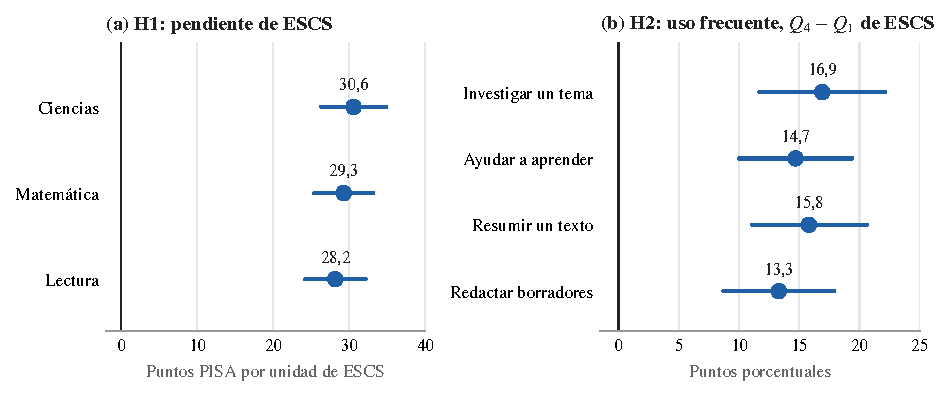
\includegraphics[width=\textwidth]{figuras/fig_h1_h2.pdf}
\caption{(a)~Pendiente del ESCS sobre el rendimiento en cada área. (b)~Diferencia entre el cuartil superior y el inferior de ESCS en la proporción que usa IA semanal o diariamente, por actividad. Puntos: estimación; líneas: IC\,95\,\%. En todas las figuras, punto lleno azul indica que el intervalo excluye el cero y punto hueco gris que lo incluye.}\label{fig:h1h2}
\end{figure}

\subsection{H2: uso de IA según nivel socioeconómico}
Entre los 7.191 estudiantes con ESCS y los cuatro ítems respondidos, la frecuencia media de uso es 0,49 puntos mayor (en la escala de 1 a 5) en el cuartil superior de ESCS que en el inferior (\ic{0,36}{0,62}). La proporción que usa IA semanal o diariamente es mayor en el cuartil superior en las cuatro actividades: 16,9\pp{} al investigar un tema, 15,8\pp{} al resumir, 14,7\pp{} al ayudar a aprender y 13,3\pp{} al redactar borradores (cuadro~\ref{tab:h1h2}; figura~\ref{fig:h1h2}b). Los cuatro intervalos excluyen el cero con holgura.

\subsection{H3: rendimiento según frecuencia de uso, sin ajustar}
El cuadro~\ref{tab:h3} y la figura~\ref{fig:h3} presentan los ocho contrastes. Quienes usan IA con frecuencia superan en ciencias a quienes nunca la usan en tres actividades: investigar un tema ($+$28,4 puntos; \ic{17,6}{39,3}), ayudar a aprender ($+$26,6; \ic{17,2}{36,0}) y resumir un texto ($+$18,8; \ic{9,4}{28,1}). Los tres contrastes superan el umbral de Bonferroni. Para redactar borradores la diferencia no es concluyente ($+$7,1; \ic{$-$3,0}{17,2}). El uso ocasional no se distingue del no uso en ninguna actividad; en redactar borradores la estimación es negativa ($-$8,5; \ic{$-$18,0}{0,9}). Como referencia de magnitud, las tres diferencias concluyentes equivalen al 35\,\%, 32\,\% y 23\,\% de la brecha de rendimiento entre cuartiles extremos de ESCS.

\begin{table}[t]
\caption{H3: diferencias de medias en ciencias según la frecuencia de uso de IA, por actividad, sin ajustar ($n=7.191$).}\label{tab:h3}
\small
\begin{threeparttable}
\begin{tabularx}{\textwidth}{@{}Xrrrrr@{}}
\toprule
Contraste y actividad & $n$ & Diferencia & EE & IC 95\,\% & $p$ \\
\midrule
\filas{tab_h3}
\bottomrule
\end{tabularx}
\begin{tablenotes}\footnotesize
\item $^{\ast}$ Supera el umbral de Bonferroni para ocho contrastes ($p<0{,}00625$). $n$ es el tamaño de la muestra analítica; cada contraste usa los estudiantes de las dos categorías comparadas.
\end{tablenotes}
\end{threeparttable}
\end{table}

\begin{figure}[t]
\centering
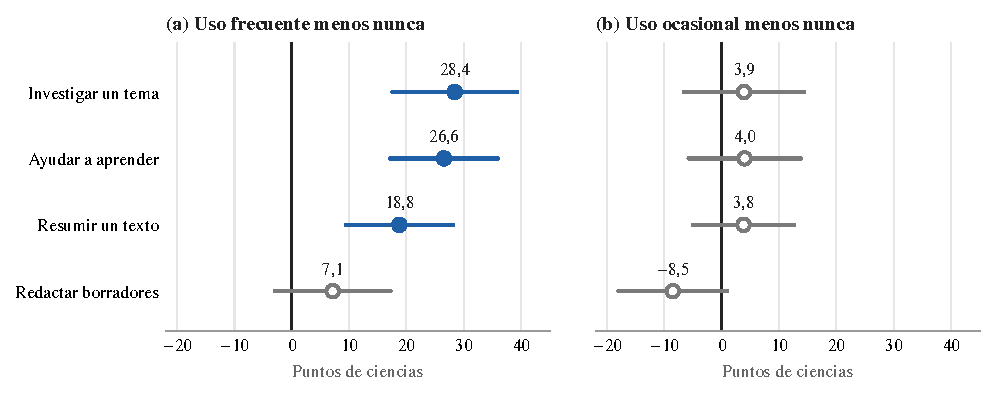
\includegraphics[width=\textwidth]{figuras/fig_h3.pdf}
\caption{H3: diferencia de medias en ciencias respecto de quienes nunca usan IA, por actividad, sin ajustar. (a)~Uso semanal o diario. (b)~Uso una o dos veces al año o al mes.}\label{fig:h3}
\end{figure}

\subsection{H4 y H5: asociación condicional e interacción}
Sin controles, cada punto adicional de frecuencia media de uso se asocia con 9,48 puntos más en ciencias (\ic{6,24}{12,72}). Al incorporar el ESCS el coeficiente baja a 5,02 (una reducción del 47\,\%) y con ESCS, sexo y grado a 4,03 (\ic{1,14}{6,92}; $p=0{,}0063$), una reducción total del 58\,\% (cuadro~\ref{tab:h4h5}; figura~\ref{fig:h4}a). Por actividad, la asociación condicional se mantiene para investigar un tema (5,24; \ic{2,61}{7,88}) y ayudar a aprender (5,55; \ic{3,22}{7,88}); para resumir un texto (1,60) y redactar borradores ($-$0,64) los intervalos incluyen el cero (figura~\ref{fig:h4}b). Resumir, que mostraba una diferencia bruta concluyente en H3, deja de distinguirse de cero al condicionar.

En cuanto a la magnitud: bajo el supuesto de linealidad, recorrer toda la escala de frecuencia (de 1 a 5) correspondería a $4\times4{,}03\approx16$ puntos, alrededor de una quinta parte de la brecha entre cuartiles extremos de ESCS.

El coeficiente de interacción entre frecuencia de uso y ESCS (H5) es $+$2,42 (\ic{$-$0,31}{5,15}; $p=0{,}082$): el signo sugiere una asociación algo mayor a mayor ESCS, pero el intervalo incluye el cero y la evidencia es insuficiente.

\begin{table}[t]
\caption{H4 y H5: coeficientes de la frecuencia de uso de IA sobre el puntaje de ciencias (puntos por punto de la escala 1--5; $n=7.191$).}\label{tab:h4h5}
\small
\begin{threeparttable}
\begin{tabularx}{\textwidth}{@{}Xrrrrr@{}}
\toprule
Modelo y regresor & $n$ & Coeficiente & EE & IC 95\,\% & $p$ \\
\midrule
\filas{tab_h4_h5}
\bottomrule
\end{tabularx}
\begin{tablenotes}\footnotesize
\item \enquote{Ajustado} sin más aclaración: controla ESCS, sexo (\var{MALE}) y grado relativo (\var{GRADE}), ecuación~\eqref{eq:h4}. $^{\dagger}$ Estimación del análisis de sensibilidad (\arch{04\_sensibilidad.csv}). El modelo de H5 es la ecuación~\eqref{eq:h5}.
\end{tablenotes}
\end{threeparttable}
\end{table}

\begin{figure}[t]
\centering
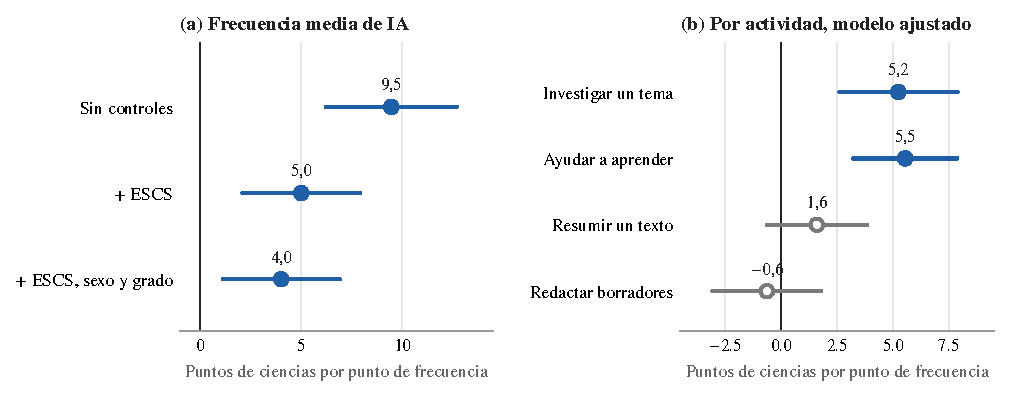
\includegraphics[width=\textwidth]{figuras/fig_h4.pdf}
\caption{H4: coeficiente de la frecuencia de uso de IA sobre ciencias. (a)~Atenuación del coeficiente de la frecuencia media al incorporar controles. (b)~Coeficiente de cada actividad en el modelo ajustado por ESCS, sexo y grado.}\label{fig:h4}
\end{figure}

\subsection{HC1: la no respuesta a las preguntas de IA}
Al preparar los datos se observó que quienes no respondieron los ítems de IA diferían de quienes sí lo hicieron (cuadro~\ref{tab:noresp}). Formalizado como hipótesis complementaria, y excluyendo a los 526 estudiantes a quienes el bloque no se administró, quienes respondieron los cuatro ítems obtienen 66,0 puntos más en ciencias que quienes no (\ic{57,7}{74,2}; $n=10.566$). Ajustando por ESCS la diferencia es de 53,8 puntos (\ic{46,4}{61,2}; $n=9.808$): el nivel socioeconómico explica una parte menor de la brecha (cuadro~\ref{tab:hc}; figura~\ref{fig:hc}a). La diferencia bruta equivale al 80\,\% de la brecha entre cuartiles extremos de ESCS y es, en puntos, la segunda mayor del estudio.

\begin{table}[t]
\caption{Comparación descriptiva entre quienes respondieron los cuatro ítems de IA ($n=7.475$) y quienes no ($n=3.617$, incluidos los 526 con bloque no administrado). Medias con el primer valor plausible; sin errores estándar.}\label{tab:noresp}
\small
\begin{threeparttable}
\begin{tabularx}{\textwidth}{@{}Xrrrrr@{}}
\toprule
 & \multicolumn{2}{c}{Sin ponderar} & \multicolumn{3}{c}{Ponderado} \\
\cmidrule(lr){2-3}\cmidrule(lr){4-6}
Variable & Respondió & No resp. & Respondió & No resp. & Diferencia \\
\midrule
\filas{tab_no_respuesta}
\bottomrule
\end{tabularx}
\begin{tablenotes}\footnotesize
\item Fuente: \arch{reports/tables/02\_comparacion\_respondieron\_ia.csv}. Esta comparación es descriptiva y difiere de HC1 (cuadro~\ref{tab:hc}), que usa los diez valores plausibles, excluye los casos no administrados e informa incertidumbre.
\end{tablenotes}
\end{threeparttable}
\end{table}

\subsection{HC2--HC4: hipótesis exploratorias registradas antes del cálculo}
\paragraph{HC2 (tipo de uso)} El índice $T$ vale en promedio 0,48, 0,49, 0,49 y 0,56 en los cuartiles de ESCS primero a cuarto. La diferencia entre extremos es $+$0,082 (\ic{$-$0,030}{0,194}; $p=0{,}15$): va en la dirección esperada pero no se distingue de cero. No hay evidencia suficiente de que el \emph{tipo} de uso varíe con el nivel socioeconómico.

\paragraph{HC3 (uso según rendimiento)} El cuartil de mayor rendimiento en ciencias usa IA semanal o diariamente en alguna actividad 16,6\pp{} más que el de menor rendimiento (\ic{11,3}{22,0}), y su frecuencia media es 0,379 puntos mayor (\ic{0,230}{0,529}). Ambos contrastes superan el umbral de Bonferroni. Es la misma asociación de H3 leída en sentido inverso, lo que subraya que la dirección es indeterminada.

\paragraph{HC4 (pendiente intraescuela)} La pendiente del ESCS sobre la frecuencia media de uso es 0,185 puntos de escala por unidad de ESCS en el total (\ic{0,139}{0,231}) y 0,080 dentro de una misma escuela (\ic{0,026}{0,134}; $p=0{,}0036$), con 404 escuelas y una mediana de 18 estudiantes por escuela en la muestra analítica. La pendiente intraescuela es el 43\,\% de la total; por la identidad~\eqref{eq:descomp}, al menos el 57\,\% de la pendiente total corresponde al componente entre escuelas (cuadro~\ref{tab:hc}; figura~\ref{fig:hc}c). Esta proporción es un cociente de estimaciones puntuales: no se estimó su error estándar ni se contrastó formalmente la diferencia entre ambas pendientes.

\begin{table}[t]
\caption{Hipótesis complementarias y exploratorias.}\label{tab:hc}
\small
\begin{threeparttable}
\begin{tabularx}{\textwidth}{@{}Xrrrrr@{}}
\toprule
Parámetro & $n$ & Estimación & EE & IC 95\,\% & $p$ \\
\midrule
\filas{tab_hc}
\bottomrule
\end{tabularx}
\begin{tablenotes}\footnotesize
\item $^{\ast}$ Supera el umbral de Bonferroni para tres hipótesis ($p<0{,}0167$). HC2--HC4: $n=7.191$ (ESCS y cuatro ítems de IA). La pendiente de HC4 se expresa en puntos de la escala 1--5 por unidad de ESCS.
\end{tablenotes}
\end{threeparttable}
\end{table}

\begin{figure}[t]
\centering
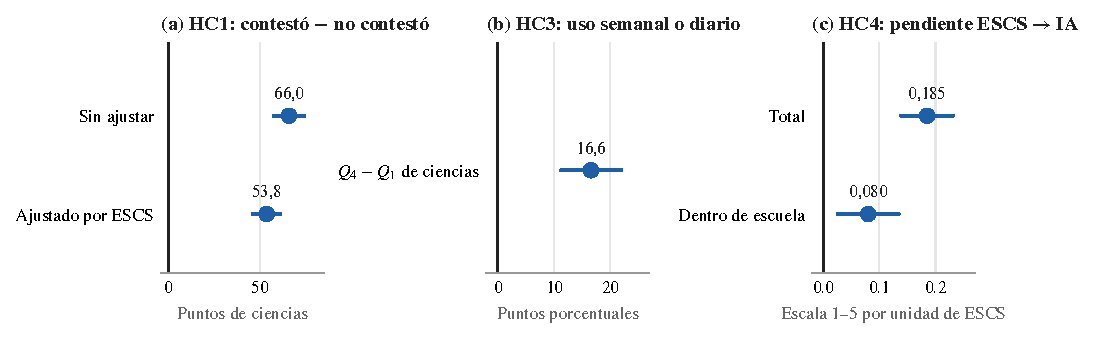
\includegraphics[width=\textwidth]{figuras/fig_exploratorias.pdf}
\caption{Hipótesis complementarias. (a)~HC1: diferencia en ciencias entre quienes respondieron los cuatro ítems de IA y quienes no. (b)~HC3: diferencia en la proporción de uso semanal o diario entre los cuartiles extremos de rendimiento en ciencias. (c)~HC4: pendiente del ESCS sobre la frecuencia media de uso, total y dentro de la escuela.}\label{fig:hc}
\end{figure}

\subsection{Análisis de sensibilidad}\label{sec:sensibilidad}
Se examinaron cuatro familias de variantes, definidas antes de calcularlas (cuadro~\ref{tab:sens}; figura~\ref{fig:sens}). (A)~\emph{Área:} el coeficiente ajustado es similar en matemática (4,19) y lectura (3,31). (B)~\emph{Medida de IA:} con el índice \var{AIUSESCH} el coeficiente es 3,61 por unidad del índice ($p=0{,}030$); con la media de los ítems respondidos, incluyendo respuestas parciales ($n=7.618$), 4,15. Usar IA semanal o diariamente en alguna actividad se asocia con $+$14,3 puntos; haber usado IA \emph{alguna vez} no se distingue de no haberlo hecho ($+$6,1; \ic{$-$6,5}{18,7}), lo que se explica porque el 91,9\,\% de la muestra analítica (6.608 de 7.191, sin ponderar) la usó alguna vez y el grupo de comparación es pequeño. (C)~\emph{Controles:} es la variante que más modifica la magnitud (9,48, 5,02 y 4,03; cuadro~\ref{tab:h4h5}). (D)~\emph{Contraste estricto:} comparar el uso diario con el no uso reproduce el patrón de H3, con diferencias positivas para ayudar a aprender ($+$26,8), investigar ($+$21,0) y resumir ($+$12,5; $p=0{,}021$) y un resultado no concluyente para redactar ($+$6,4).

En suma, el signo positivo y el orden entre actividades son estables; la magnitud depende sobre todo de los controles. Las variantes con otra métrica (binaria o índice) no son comparables en tamaño con el coeficiente de referencia, solo en signo y significación.

\begin{table}[t]
\caption{Análisis de sensibilidad. Los bloques A y B usan el modelo ajustado por ESCS, sexo y grado; el bloque D son diferencias de medias sin ajustar.}\label{tab:sens}
\small
\begin{threeparttable}
\begin{tabularx}{\textwidth}{@{}Xrrrrr@{}}
\toprule
Variante & $n$ & Estimación & EE & IC 95\,\% & $p$ \\
\midrule
\filas{tab_sensibilidad}
\bottomrule
\end{tabularx}
\begin{tablenotes}\footnotesize
\item El bloque C (controles) se presenta en el cuadro~\ref{tab:h4h5}. Ninguna estimación de esta tabla lleva corrección por multiplicidad.
\end{tablenotes}
\end{threeparttable}
\end{table}

\begin{figure}[t]
\centering
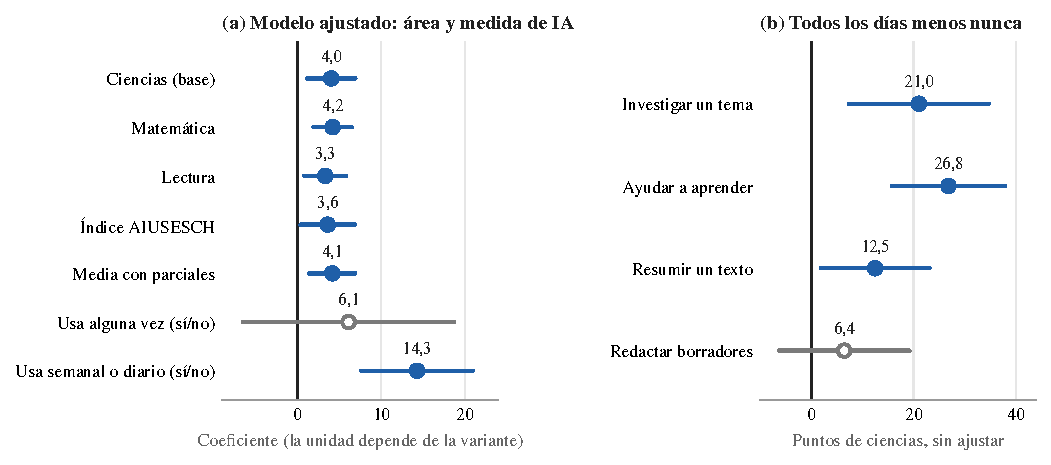
\includegraphics[width=\textwidth]{figuras/fig_sensibilidad.pdf}
\caption{Análisis de sensibilidad. (a)~Coeficiente ajustado según el área evaluada y la medida de uso de IA; las unidades difieren entre variantes. (b)~Diferencia en ciencias entre quienes usan IA todos los días y quienes nunca la usan, por actividad, sin ajustar.}\label{fig:sens}
\end{figure}

% =====================================================================
\section{Discusión}\label{sec:discusion}

\subsection{Una brecha de uso alineada con la brecha de origen}
El resultado más firme es la coexistencia de dos gradientes socioeconómicos: uno en el rendimiento (H1), grande y estable entre áreas, y otro en la frecuencia de uso de IA (H2), presente en las cuatro actividades. La ausencia de evidencia de que el \emph{tipo} de uso cambie con el ESCS (HC2) sugiere, con la cautela que impone un resultado no concluyente, que la diferencia observable con este instrumento es de intensidad más que de finalidad. Esto es coherente con la literatura sobre brecha digital de segundo nivel \parencite{hargittai2002,vandeursen2019}, aunque el instrumento de PISA ---cuatro ítems de frecuencia--- es demasiado grueso para captar diferencias cualitativas de uso como las que resultan decisivas en la evidencia experimental \parencite{bastani2025}.

\subsection{Qué queda de la asociación entre IA y rendimiento}
La comparación bruta entre usuarios frecuentes y no usuarios (H3) arroja diferencias de 19 a 28 puntos, pero más de la mitad del coeficiente lineal desaparece al condicionar por tres variables de contexto (H4). Tres lecturas son compatibles con el coeficiente residual de 4 puntos por punto de frecuencia, y los datos no permiten discriminar entre ellas: (i)~confusión residual por características no observadas del estudiante, la familia o la escuela; (ii)~causalidad inversa ---los estudiantes de mejor desempeño adoptan más estas herramientas---, que HC3 hace visible al mostrar la misma asociación con los roles invertidos, y (iii)~algún beneficio de ciertos usos. El patrón por actividad es informativo como descripción: las actividades en las que la herramienta interviene en la comprensión (investigar, ayudar a aprender) conservan una asociación condicional positiva, mientras que aquella en la que produce texto (redactar borradores) no muestra asociación en ninguna especificación. Sería un error leer este contraste como evidencia de que unos usos \enquote{sirven} y otros no: también puede reflejar qué estudiantes eligen cada uso.

En términos de relevancia práctica, el coeficiente ajustado es modesto: toda la escala de frecuencia equivale, bajo linealidad, a una quinta parte de la brecha entre cuartiles extremos de ESCS, y su significación estadística es la más frágil de las hipótesis confirmatorias (apéndice~\ref{ap:multiplicidad}).

\subsection{La no respuesta como resultado sustantivo}
Que casi tres de cada diez estudiantes que recibieron el bloque de IA no lo respondieran, y que ese grupo rinda 66 puntos menos, no es solo una limitación técnica. Indica que la población para la cual PISA~2025 puede describir el uso de IA en Argentina está desplazada hacia arriba en rendimiento y en ESCS. Si la no respuesta se asocia con el propio uso de IA ---algo que los datos no permiten saber---, las prevalencias y las brechas estimadas entre respondentes pueden diferir de las poblacionales en una dirección desconocida \parencite{groves2006}. La brecha de respuesta se reduce poco al ajustar por ESCS, lo que sugiere que se vincula con otros factores (por ejemplo, la extensión o posición del bloque en el cuestionario, la fatiga o la comprensión lectora), hipótesis que este trabajo no evaluó.

\subsection{La escuela como lugar de la brecha}
Dentro de una misma escuela la pendiente del ESCS sobre el uso de IA es menos de la mitad que en el total (HC4). Dado que la segregación socioeconómica entre escuelas hace que buena parte de la variación del ESCS ocurra entre establecimientos, esto ubica la mayor parte de la brecha de uso en \emph{a qué escuela se asiste} más que en diferencias entre compañeros. El resultado es descriptivo: no distingue entre políticas o recursos de la escuela, composición del alumnado y normas de pares.

\subsection{Implicancias}
Para la comunidad educativa, la conclusión prudente es doble. Primero, cualquier política sobre IA en la escuela opera sobre un uso ya extendido entre quienes responden (en la muestra analítica, sin ponderar, más de nueve de cada diez declaran haberla usado alguna vez) y ya desigual. Segundo, los datos transversales no permiten recomendar ni desaconsejar el uso por sus consecuencias sobre el aprendizaje: para eso se requieren diseños longitudinales o experimentales.

% =====================================================================
\section{Limitaciones y amenazas a la validez}\label{sec:limitaciones}

\paragraph{Validez interna: no hay identificación causal} El diseño es transversal y observacional. Ningún coeficiente debe leerse como efecto del uso de IA ni del nivel socioeconómico. Los controles disponibles en el modelo son tres; el cuestionario de PISA contiene otras covariables que no se utilizaron y con las cuales el coeficiente de H4 podría reducirse más.

\paragraph{Validez externa: no respuesta selectiva} Las hipótesis H2 a H5 y HC2 a HC4 se estiman sobre el 64,8\,\% de la muestra. Los pesos finales de PISA ajustan la no respuesta de escuelas y estudiantes a la evaluación, no la no respuesta a ítems del cuestionario; no se reponderó ni se imputó, y no se realizó un análisis de sensibilidad a mecanismos de no respuesta no ignorables. En consecuencia, todos los resultados sobre IA describen a quienes respondieron. Además, los cuartiles de ESCS se definieron sobre los 9.808 estudiantes con ESCS válido, de modo que en la submuestra de 7.191 no representan cuartos iguales de la población.

\paragraph{Validez de constructo} El uso de IA es autodeclarado y se limita a la frecuencia de cuatro actividades con chatbots; no mide calidad, intensidad, finalidad ni integridad académica. La categoría \enquote{ocasional} reúne frecuencias anuales y mensuales. La frecuencia media $\bar A$ trata una escala ordinal como intervalar. El ESCS es un índice relativo, no ingreso. Los valores plausibles se generan con un modelo de condicionamiento; si las variables de IA no forman parte de ese modelo, las asociaciones con ellas pueden estar atenuadas \parencite{mislevy1991}, cuestión que no se pudo verificar en la documentación provisional.

\paragraph{Validez de la conclusión estadística} (i)~El factor de Fay $k=0{,}5$ no está confirmado para PISA~2025 (sección~\ref{sec:fay}). (ii)~Los cortes de los cuartiles de ESCS se fijaron con el peso final y no se recalcularon en cada réplica, por lo que los errores estándar de los contrastes entre cuartiles no incluyen la variabilidad de los cortes (sí lo hacen en HC3). (iii)~Los valores $p$ usan la referencia normal. (iv)~Solo H3 y HC2--HC4 llevan corrección por multiplicidad; se informaron 46 estimaciones en total. (v)~No se informan tamaños de efecto estandarizados ni medidas de ajuste de los modelos. (vi)~El modelo de H4 supone linealidad en la frecuencia media; H3 muestra que la relación bruta no es lineal (el uso ocasional no difiere del no uso), de modo que el coeficiente lineal resume una relación concentrada en el extremo superior de la escala.

\paragraph{Verificación del cómputo} La documentación del proyecto (\arch{docs/estado.md}) registra que una segunda implementación, escrita aparte sobre los mismos datos, reprodujo cuatro resultados centrales con diferencias menores que 0,01. Ese código no está versionado en el repositorio, por lo que la comprobación no es reproducible por terceros. Los resultados no se contrastaron con software estadístico especializado en encuestas \parencite[p.~ej.,][]{lumley2010}. Durante la preparación de este manuscrito no se dispuso de los microdatos, de modo que las cifras se tomaron de las salidas ejecutadas y versionadas, cuya coherencia interna se comprobó (apéndice~\ref{ap:trazabilidad}), pero el análisis no se volvió a ejecutar.

\paragraph{Discrepancias detectadas al auditar el proyecto} El cuadro~\ref{tab:auditoria} (apéndice~\ref{ap:auditoria}) lista las diferencias encontradas entre la documentación del proyecto y lo efectivamente implementado, y cómo se tratan aquí. Ninguna altera una estimación; dos afectan la redacción de conclusiones del informe original y se corrigen en este texto.

\paragraph{Alcance de la revisión bibliográfica} Los antecedentes no provienen de una búsqueda sistemática. No se buscaron de manera exhaustiva análisis previos de las preguntas de IA de PISA~2025, por lo que no se afirma que los resultados sean novedosos.

% =====================================================================
\section{Conclusiones y líneas futuras}\label{sec:conclusiones}

Con el diseño muestral completo de PISA~2025, este trabajo encuentra en Argentina (i)~una asociación grande entre nivel socioeconómico y rendimiento (30,6 puntos de ciencias por unidad de ESCS; 82,4 puntos entre cuartiles extremos); (ii)~una brecha socioeconómica en el uso frecuente de chatbots de IA de 13 a 17 puntos porcentuales entre quienes respondieron; (iii)~una asociación positiva entre uso frecuente y rendimiento que se reduce en un 58\,\% al ajustar por ESCS, sexo y grado, queda en 4,0 puntos por punto de frecuencia y se sostiene solo para investigar un tema y ayudar a aprender; (iv)~evidencia insuficiente de que esa asociación varíe con el ESCS o de que el tipo de uso difiera entre niveles socioeconómicos, y (v)~una no respuesta del 29\,\% a las preguntas de IA, concentrada en estudiantes de rendimiento mucho menor. La pendiente socioeconómica del uso se reduce a menos de la mitad dentro de una misma escuela.

La respuesta a la pregunta de investigación es, por lo tanto, asimétrica: PISA~2025 permite afirmar con solidez que el uso de IA está socialmente estratificado entre quienes informan sobre él, y permite afirmar muy poco sobre sus consecuencias para el aprendizaje.

\paragraph{Líneas futuras (no ejecutadas)} Las siguientes extensiones se proponen y \emph{no} forman parte de los resultados: (1)~caracterizar la no respuesta al bloque de IA y evaluar la sensibilidad de H2--H4 a mecanismos de no respuesta alternativos (reponderación, imputación múltiple, cotas); (2)~estimar $\rho$ y $b_B$ en la identidad~\eqref{eq:descomp} y vincular la brecha entre escuelas con el cuestionario de escuelas, que se descargó pero no se analizó; (3)~recalcular los cuartiles de ESCS en cada réplica, informar tamaños de efecto estandarizados y contrastar el estimador con software de terceros; (4)~confirmar el factor de replicación cuando se publique el informe técnico final de PISA~2025; (5)~ampliar los controles y examinar la no linealidad de la relación; (6)~comparar con otros países y con ciclos futuros, y (7)~abordar la pregunta causal con diseños longitudinales o experimentales.

% =====================================================================
\section*{Disponibilidad de datos y código}
\addcontentsline{toc}{section}{Disponibilidad de datos y código}
El código, las tablas de resultados, las figuras y los archivos fuente de este manuscrito están en el repositorio \url{https://github.com/nazareno-urday/pisa-analysis-argentina}, bajo licencia MIT. Los microdatos de PISA no se redistribuyen: se obtienen de la OCDE \parencite{oecd2025db} y deben ubicarse según indica el \arch{README.md}. Las condiciones de uso y la atribución exigidas por la OCDE figuran como \emph{no verificadas} en \arch{docs/fuentes\_y\_licencias.md} y deben confirmarse antes de la publicación. La carpeta \arch{paper/} contiene los programas que generan los cuadros y las figuras del artículo a partir de las tablas versionadas.

\section*{Declaraciones}
\addcontentsline{toc}{section}{Declaraciones}
\noindent\textbf{Ética.} El estudio es un análisis secundario de un archivo de uso público, sin identificadores personales; no se recolectaron datos nuevos ni se intentó reidentificar individuos o escuelas.\\
\textbf{Uso de herramientas de inteligencia artificial.} La redacción de este manuscrito, la generación de sus cuadros y figuras a partir de las salidas versionadas y la auditoría de coherencia contaron con la asistencia de un asistente de IA generativa; ello no constituye revisión por pares ni revisión externa. El autor es responsable del contenido. \pendiente{indicar si también hubo asistencia de IA en el desarrollo del análisis y nombrar las herramientas, según la política de la revista.}\\
\textbf{Financiamiento.} \pendiente{declarar la fuente de financiamiento o su ausencia.}\\
\textbf{Conflictos de interés.} \pendiente{declarar.}\\
\textbf{Afiliación y contacto.} \pendiente{completar si corresponde; no se incluyó ninguna por no constar en el proyecto.}

\printbibliography[title={Referencias}]

% =====================================================================
\appendix
\section{Descomposición de la pendiente total}\label{ap:descomposicion}
Sean $x_i$ e $y_i$ dos variables, $w_i$ los pesos, $\bar x$ e $\bar y$ sus medias ponderadas globales y $\bar x_j$, $\bar y_j$ las medias ponderadas en la escuela $j$, con $W_j=\sum_{i\in j}w_i$. Escribiendo $x_i-\bar x=(x_i-\bar x_{j(i)})+(\bar x_{j(i)}-\bar x)$ y análogamente para $y$, y observando que $\sum_{i\in j}w_i(x_i-\bar x_j)=0$ para toda escuela, los productos cruzados se anulan y
\[
S_{xy}=\underbrace{\sum_i w_i(x_i-\bar x_{j(i)})(y_i-\bar y_{j(i)})}_{S_{xy}^{W}}
+\underbrace{\sum_j W_j(\bar x_j-\bar x)(\bar y_j-\bar y)}_{S_{xy}^{B}},
\]
con la misma descomposición para $S_{xx}$. Definiendo $b_W=S_{xy}^{W}/S_{xx}^{W}$, $b_B=S_{xy}^{B}/S_{xx}^{B}$ y $\rho=S_{xx}^{B}/S_{xx}$,
\[
b_T=\frac{S_{xy}}{S_{xx}}=\frac{S_{xx}^{W}}{S_{xx}}\,b_W+\frac{S_{xx}^{B}}{S_{xx}}\,b_B=(1-\rho)\,b_W+\rho\,b_B .
\]
La fracción de $b_T$ correspondiente al componente entre escuelas es $\rho\,b_B/b_T=1-(1-\rho)\,b_W/b_T$. Como $0\le1-\rho\le1$, si $b_W/b_T\ge0$ esa fracción es al menos $1-b_W/b_T$. Con $b_T=0{,}185$ y $b_W=0{,}080$ la cota es $1-0{,}432=0{,}568$. La identidad es exacta para las estimaciones calculadas con el peso final sobre la misma muestra; la cota hereda la incertidumbre de ambas pendientes, que no se cuantificó para el cociente.

\section{Multiplicidad y distribución de referencia}\label{ap:multiplicidad}
Esta sección no contiene estimaciones nuevas: aplica criterios alternativos a los valores $p$ y errores estándar ya publicados en las tablas del proyecto (cálculo en \arch{paper/tablas.py}; salida en \arch{paper/verificacion\_cifras.txt}). Se presenta separada de los resultados originales porque no formaba parte del plan de análisis.

\paragraph{Familia H4.} Si las seis estimaciones de H4 se trataran como una familia ($\alpha/6=0{,}0083$), cuatro superarían el umbral: el coeficiente sin ajustar, el ajustado de la frecuencia media ($p=0{,}0063$) y los de investigar un tema y ayudar a aprender.

\paragraph{Todas las estimaciones.} Las tres tablas contienen 46 filas (43 estimaciones distintas, porque el modelo de referencia se repite). Con un umbral de Bonferroni global ($0{,}05/46=0{,}0011$), 25 filas lo superan. Entre las que tienen $p<0{,}05$ pero no lo superan están el coeficiente ajustado de H4 ($p=0{,}0063$), la pendiente intraescuela de HC4 ($p=0{,}0036$), los coeficientes ajustados en lectura y con el índice \var{AIUSESCH}, y los contrastes estrictos de investigar y resumir. Todas las estimaciones de H1 y H2, los tres contrastes concluyentes de H3, HC1, HC3 y la pendiente total de HC4 lo superan. El criterio global es deliberadamente conservador; se informa para mostrar qué conclusiones no dependen de la elección de familia.

\paragraph{Referencia $t$ en lugar de normal.} Con una $t$ de Student de 80 grados de libertad (cota superior razonable para 80 réplicas), el valor crítico bilateral al 5\,\% es $1{,}990$. Ningún veredicto al nivel $0{,}05$ cambia en las 46 filas. Para los tres resultados más cercanos a sus umbrales: H4 ajustado, $p=0{,}0077$ (umbral $0{,}05$); pendiente intraescuela de HC4, $p=0{,}0055$ (umbral $0{,}0167$); H3 resumir, $p=0{,}00017$ (umbral $0{,}00625$).

\section{Trazabilidad de los resultados}\label{ap:trazabilidad}
\begin{table}[h!]
\caption{Origen de cada resultado. Los cuadernos están en \arch{notebooks/} y las tablas en \arch{reports/tables/}.}\label{tab:trazabilidad}
\small
\begin{tabularx}{\textwidth}{@{}>{\raggedright\arraybackslash}p{4.3cm}>{\raggedright\arraybackslash}X>{\raggedright\arraybackslash}p{4.4cm}@{}}
\toprule
Resultado & Cuaderno y sección & Archivo de salida \\
\midrule
Tamaños del archivo, cobertura, PISA~2022 & \arch{00\_viabilidad\_y\_fuentes}, §3--6 & Salidas del cuaderno \\
Códigos de faltante, duplicados, rangos & \arch{01\_carga\_y\_comprension}, §3--5 & \arch{docs/diccionario\_datos.csv} \\
Muestras analíticas, cortes de ESCS & \arch{02\_preparacion}, §3--4 & \arch{02\_exclusiones.csv} \\
Comparación respondió / no respondió & \arch{02\_preparacion}, §5 & \arch{02\_comparacion\_respondieron\_ia.csv} \\
Estimador de varianza y prueba & \arch{03\_exploracion\_e\_hipotesis}, §1 & Salidas del cuaderno \\
H1--H5 y HC1 & \arch{03\_exploracion\_e\_hipotesis}, §3--8 & \arch{03\_resultados\_hipotesis.csv} \\
Medias de ciencias por cuartil & \arch{03\_exploracion\_e\_hipotesis}, §3 & Salida de la celda de la figura \\
Sensibilidad A--D & \arch{04\_sensibilidad\_y\_evaluacion}, §3--6 & \arch{04\_sensibilidad.csv} \\
HC2--HC4 & \arch{05\_hipotesis\_exploratorias}, §2--4 & \arch{05\_hipotesis\_exploratorias.csv} \\
Cuadros y figuras de este artículo & \arch{paper/tablas.py}, \arch{paper/figuras.py} & \arch{paper/tablas/}, \arch{paper/figuras/} \\
Cocientes derivados y apéndice~\ref{ap:multiplicidad} & \arch{paper/tablas.py} & \arch{paper/verificacion\_cifras.txt} \\
\bottomrule
\end{tabularx}
\end{table}

El programa \arch{paper/tablas.py} recalcula, para las 46 filas, los límites del intervalo y el estadístico $z$ a partir de la estimación y el error estándar publicados, y se detiene con error si no coinciden con los valores guardados dentro de la tolerancia de redondeo. Esta comprobación detecta errores de transcripción o tablas alteradas; no verifica que las estimaciones sean correctas respecto de los microdatos.

\section{Discrepancias entre la documentación y la implementación}\label{ap:auditoria}
\begin{table}[h!]
\caption{Observaciones de la auditoría del proyecto realizada al preparar el manuscrito.}\label{tab:auditoria}
\small
\begin{tabularx}{\textwidth}{@{}>{\raggedright\arraybackslash}p{0.5cm}>{\raggedright\arraybackslash}X>{\raggedright\arraybackslash}X@{}}
\toprule
N.º & Observación & Impacto y tratamiento en este artículo \\
\midrule
1 & La tabla de exclusiones asigna a \enquote{H3 sin ajustar} la muestra de 7.475 estudiantes con los cuatro ítems de IA; el código estima H3 sobre los 7.191 que además tienen ESCS. & Las cifras de H3 corresponden a $n=7.191$, como indica la tabla de resultados. No existe una estimación de H3 con 7.475. Se informa 7.191. \\
2 & El informe del proyecto afirma que \enquote{más de la mitad} de la asociación IA--rendimiento desaparece al ajustar por nivel socioeconómico. & Con ESCS solo, la reducción es del 47\,\%; supera la mitad (58\,\%) al añadir sexo y grado. Se corrige la redacción. \\
3 & El informe afirma que \enquote{más de la mitad de la brecha de uso se da entre escuelas} a partir del cociente $b_W/b_T=0{,}43$, sin justificación formal. & La afirmación es correcta como cota inferior para las estimaciones puntuales (apéndice~\ref{ap:descomposicion}), pero sin medida de incertidumbre. Se presenta así. \\
4 & En H5 las variables se centran en la media \emph{sin ponderar} de la muestra analítica. & El coeficiente de interacción es invariante al centrado. El coeficiente principal de IA se interpreta en la media muestral no ponderada del ESCS, no en la poblacional. \\
5 & Los cuartiles de ESCS se calculan sobre 9.808 casos y se reutilizan en la submuestra de 7.191. & Los grupos $Q_1$ y $Q_4$ de H2 y HC2 no son cuartos exactos de esa submuestra. Se declara como limitación. \\
6 & La validación con una segunda implementación se menciona en la documentación, pero su código no está en el repositorio. & Se informa como comprobación no reproducible por terceros. \\
7 & La comparación descriptiva de la tabla \arch{02\_comparacion} incluye en \enquote{no respondieron} a los 526 casos no administrados; HC1 los excluye. & Se presentan por separado (cuadros~\ref{tab:noresp} y~\ref{tab:hc}) y se explicita la diferencia. \\
8 & Los términos de uso de los datos de la OCDE y el factor de replicación de 2025 figuran como no verificados. & Se mantienen como pendientes explícitos. \\
\bottomrule
\end{tabularx}
\end{table}

\end{document}
